\chapter{Subtracting $\gamma$-ray background}
\label{appendix:bg_subtraction}

\begin{figure}[h!]
    \centering
      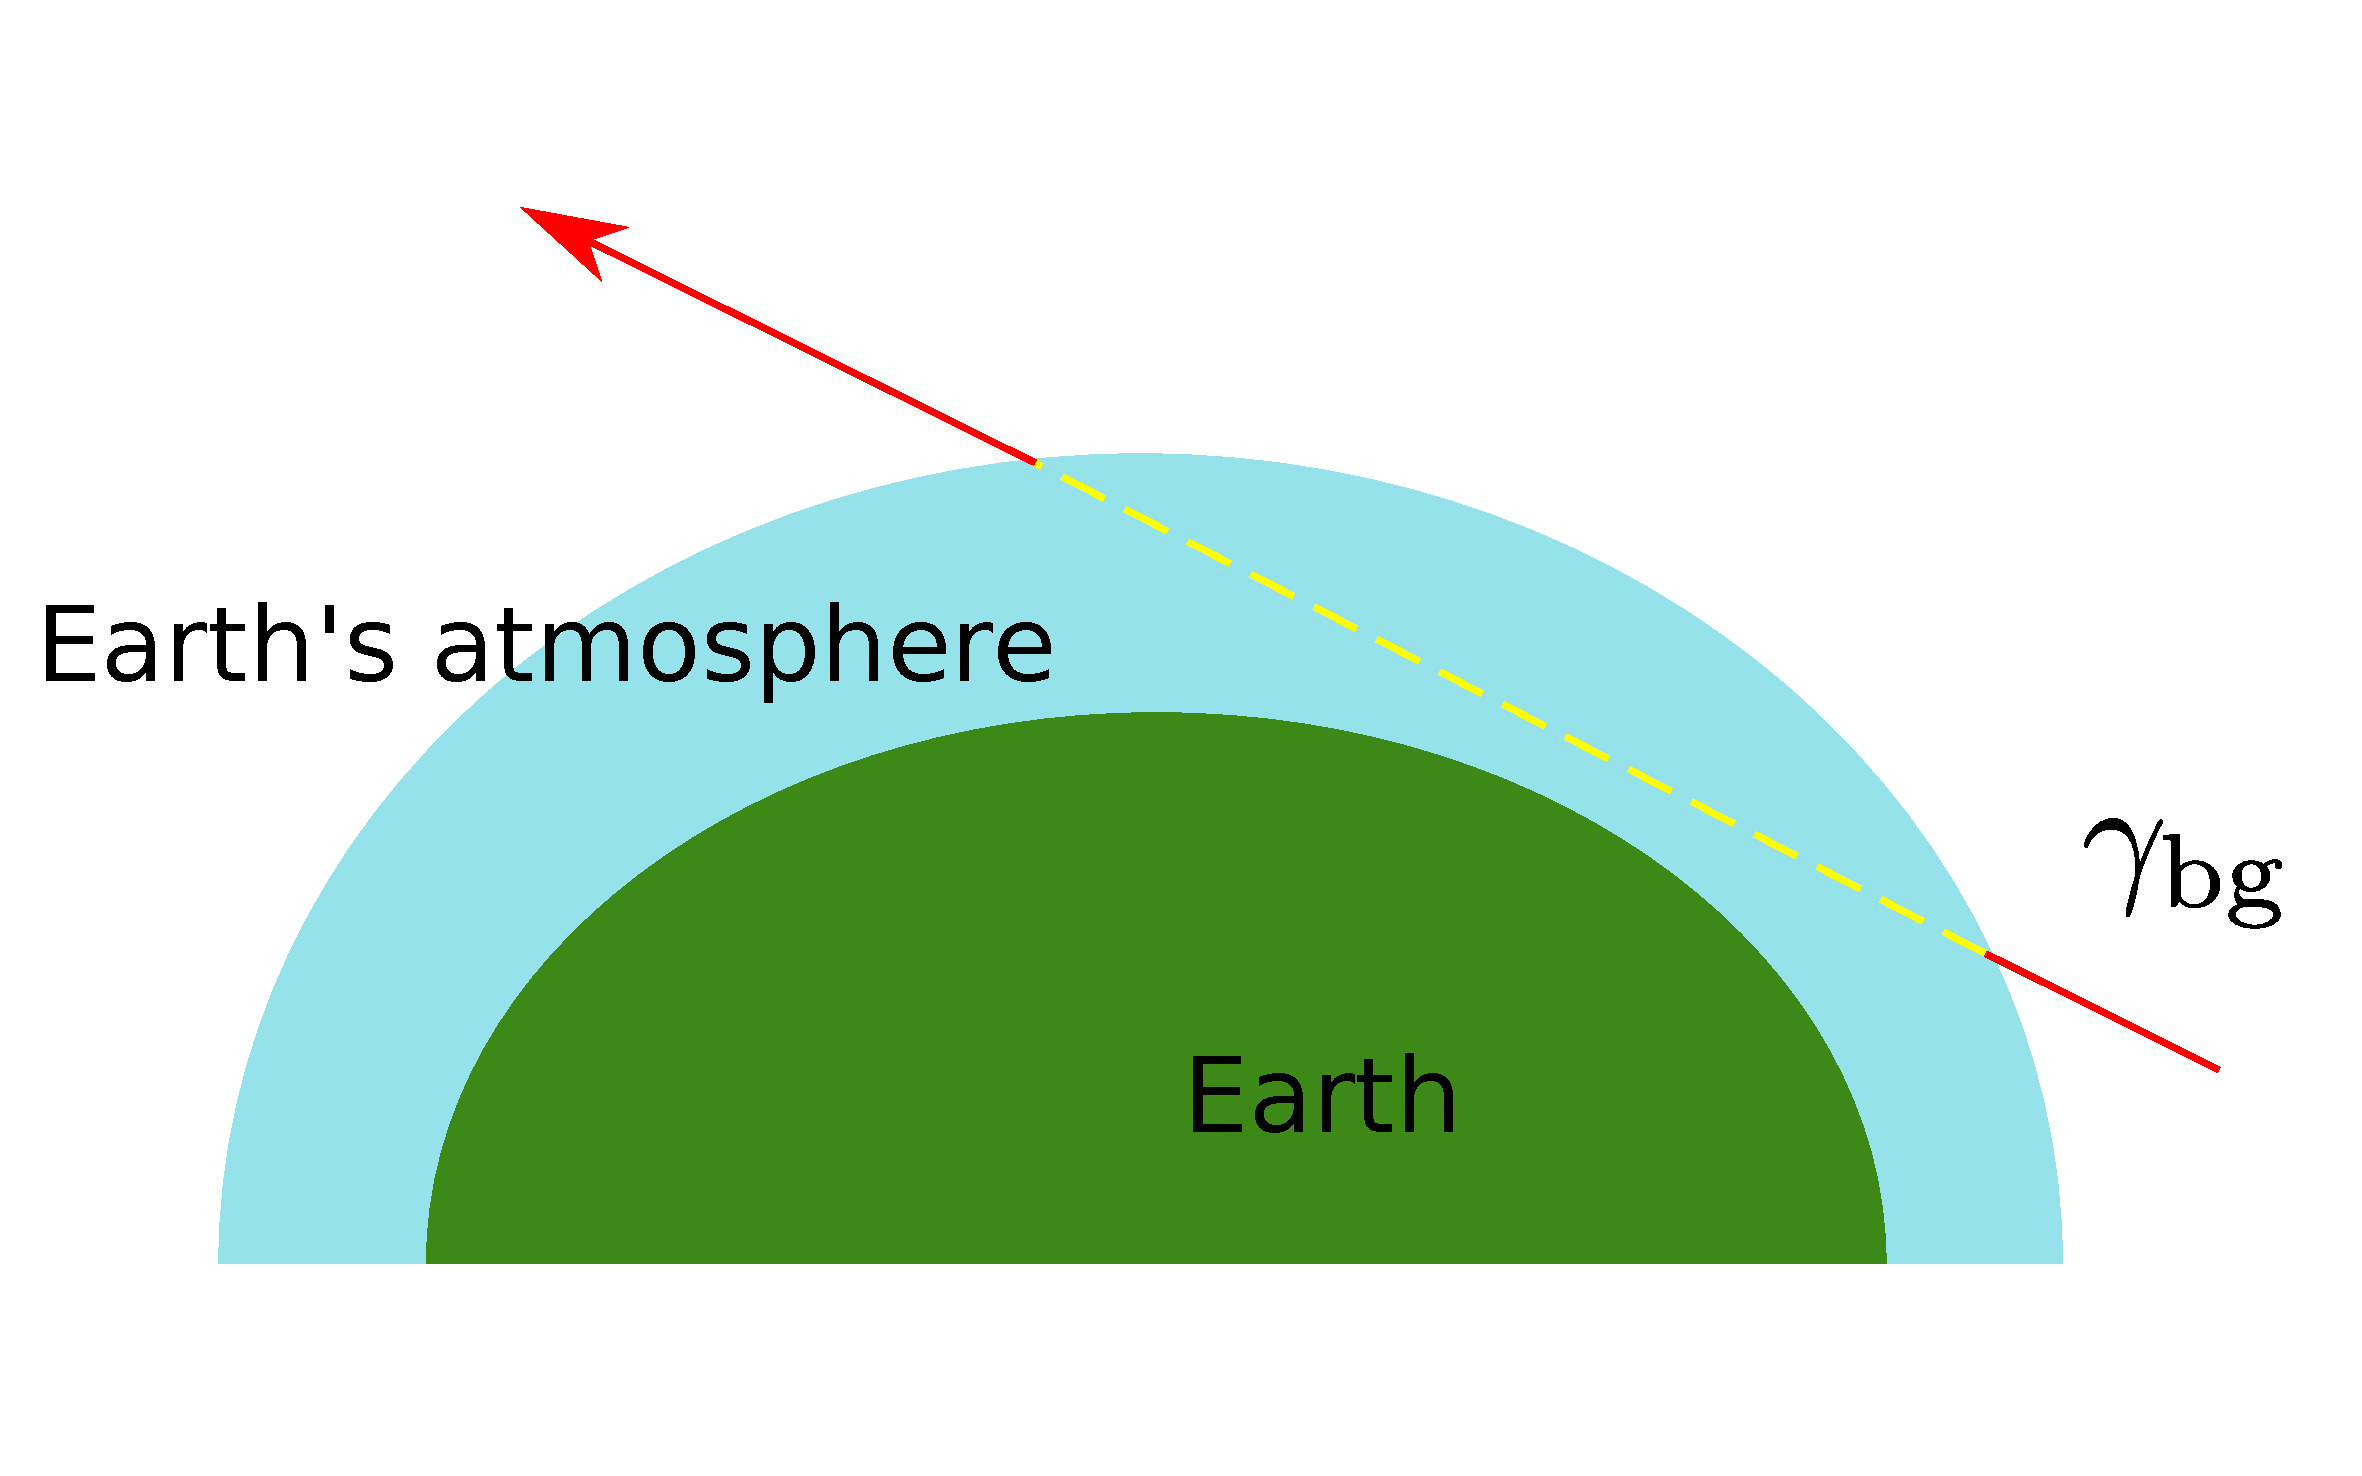
\includegraphics[width=0.6\textwidth]{appendix/bg_subtraction/backgroundSubtract.pdf}
      \caption{Schematics of $\gamma$-ray propagation from diffusive background}
\end{figure}


Assuming
the classical collision process, we obtain
% the probability of the collision process as a classical relation 

\begin{equation}
    N \equiv N_0 e^{-n\sigma x}
\end{equation}
when
\begin{itemize}
    \item $N$ is the surviving number of photons
    \item $N_0$ is the original number of photons    
    \item $n$ is a density of the air
    \item $\sigma$ is a crossection of the $\gamma$-ray and the air
    \item $x$ is a propagation length.
\end{itemize}
% XCOM:NIST(2010) 
From using cross-section data from \cite{XCOMNIST},
we find that collision probability of a $\gamma$-ray
with a nitrogen atom and
that with an oxygen atom are
% oxygen atom very
similar in
the energy range of our interest.
If we consider a worst-case scenario 
(longest path and highest density that could happen in 
the upper atmosphere of our interest),
we
find that the possibility of a diffuse background
photon passing through approaches one. 
Therefore, we can straightforwardly remove the background
contamination by using an estimation from the average sky
diffusive intensity.
% found a passing possibility approach to one more than third order.
% To sum up, we could straightforwardly remove background by taking
% the average diffusive background per unit of angle before applying.

